\documentclass{article}



\usepackage[dutch]{babel}
\usepackage[utf8x]{inputenc}
\usepackage[margin=3cm]{geometry}
\usepackage{graphicx}
\usepackage{hyperref}
\usepackage{float}
\usepackage{booktabs}
\usepackage{caption}
\usepackage{hhline}
\usepackage[parfill]{parskip}
\usepackage{xcolor}
\usepackage{amsmath}
\usepackage{hyphenat}

% fonts
\usepackage[T1]{fontenc}
\usepackage{helvet}
\renewcommand{\familydefault}{\sfdefault}

%Define the listing package
\usepackage{listings} %code highlighter
\usepackage{color} %use color
\definecolor{mygreen}{rgb}{0,0.6,0}
\definecolor{mygray}{rgb}{0.5,0.5,0.5}
\definecolor{mymauve}{rgb}{0.58,0,0.82}
 
%Customize a bit the look
\lstset{ %
backgroundcolor=\color{white}, % choose the background color; you must add \usepackage{color} or \usepackage{xcolor}
basicstyle=\footnotesize, % the size of the fonts that are used for the code
breakatwhitespace=false, % sets if automatic breaks should only happen at whitespace
breaklines=true, % sets automatic line breaking
captionpos=b, % sets the caption-position to bottom
commentstyle=\color{mygreen}, % comment style
deletekeywords={...}, % if you want to delete keywords from the given language
escapeinside={\%*}{*)}, % if you want to add LaTeX within your code
extendedchars=true, % lets you use non-ASCII characters; for 8-bits encodings only, does not work with UTF-8
frame=single, % adds a frame around the code
keepspaces=true, % keeps spaces in text, useful for keeping indentation of code (possibly needs columns=flexible)
keywordstyle=\color{blue}, % keyword style
% language=Octave, % the language of the code
morekeywords={*,...}, % if you want to add more keywords to the set
numbers=left, % where to put the line-numbers; possible values are (none, left, right)
numbersep=5pt, % how far the line-numbers are from the code
numberstyle=\tiny\color{mygray}, % the style that is used for the line-numbers
rulecolor=\color{black}, % if not set, the frame-color may be changed on line-breaks within not-black text (e.g. comments (green here))
showspaces=false, % show spaces everywhere adding particular underscores; it overrides 'showstringspaces'
showstringspaces=false, % underline spaces within strings only
showtabs=false, % show tabs within strings adding particular underscores
stepnumber=1, % the step between two line-numbers. If it's 1, each line will be numbered
stringstyle=\color{mymauve}, % string literal style
tabsize=2, % sets default tabsize to 2 spaces
title=\lstname % show the filename of files included with \lstinputlisting; also try caption instead of title
}
%END of listing package%
 
\definecolor{darkgray}{rgb}{.4,.4,.4}
\definecolor{purple}{rgb}{0.65, 0.12, 0.82}

%define Javascript language
\lstdefinelanguage{JavaScript}{
keywords={typeof, new, true, false, catch, function, return, null, catch, switch, var, if, in, while, do, else, case, break, const, for, of, \$},
keywordstyle=\color{blue}\bfseries,
ndkeywords={class, export, boolean, throw, implements, import, this},
ndkeywordstyle=\color{darkgray}\bfseries,
identifierstyle=\color{black},
sensitive=false,
comment=[l]{//},
morecomment=[s]{/*}{*/},
commentstyle=\color{purple}\ttfamily,
stringstyle=\color{red}\ttfamily,
morestring=[b]',
morestring=[b]"
}
 
\lstset{
language=JavaScript,
extendedchars=true,
basicstyle=\footnotesize\ttfamily,
showstringspaces=false,
showspaces=false,
numbers=left,
numberstyle=\footnotesize,
numbersep=9pt,
tabsize=2,
breaklines=true,
showtabs=false,
captionpos=b
}

\newcommand{\bold}[1]{\textbf{#1}}

\begin{document}

\begin{titlepage}
    \author{Tuur Vanhoutte}
    \title{Full Stack Web Development}
\end{titlepage}

\pagenumbering{gobble}
\maketitle
\newpage
\tableofcontents
\newpage

\pagenumbering{arabic}

\section {Client-server}

\subsection{Waarmee werkt een full-stack web developer?}
\begin{itemize}
    \item Hardware  
    \item Databases
    \item API/back-end code: de logica
    \item Front-end code: visuele schil
    \item Project management
    \item \dots
\end{itemize}

\subsection{We splitsen een applicatie in 3 delen:}
\begin{enumerate}
    \item Front-end
    \begin{itemize}
        \item toont de data aan de gebruiker
        \item HTML, CSS, Javascript
    \end{itemize}
    \item Back-end 
    \begin{itemize}
        \item haalt data uit de DB, verwerkt deze en geeft de nodige data terug aan de frontend
        \item PHP, Python
    \end{itemize}
    \item Database
    \begin{itemize}
        \item opslag van alle data 
        \item SQL-server, MySQL, MariaDB
    \end{itemize}
\end{enumerate}

\subsection{Nood aan communicatie tussen 3 (verschillende) machines}
\begin{itemize}
    \item Front-end op de client
    \item Back-end op de webserver
    \item Data op de database(server)
\end{itemize}


\subsection {Webserver}
Webserver levert 'served' inhoud aan clients
\subsubsection{Verschillende producten:}
\begin{itemize}
    \item Apache (since 1995)
    \item Ngingx (since 2004)
    \item IIS (since 1995)
\end{itemize}

\subsection {TCP/IP}

\begin{itemize}
    \item Communicatie tussen de verschillende machines
    \item Fundament van client-server technologie
    \item Zorgt voor de verbinding
    \item Zegt niets over de aard en inhoud van de data: welke data/structuur/volgorde/...
    \item Zegt wel:
    \begin{itemize}
        \item Afspraken over hoe de communicatie verloopt
        \item HTTP(S), (S)FTP SMTP, POP3, IMAP, \dots
    \end{itemize}
\end{itemize}


\subsubsection{Stappenplan}
\begin{enumerate}
    \item Server zet IP en poort open
    \item Server wacht op request
    \item Client stuurt request naar IP:POORT
    \item Server accepteert connectie
    \item Data overdracht
\end{enumerate}

\subsubsection{TCP}
= Transfer Control Protocol

\begin{itemize}
    \item Poorten
    \item Bepaalt het communicatiekanaal voor een specifieke applicatie
    \item Server kan adhv poort beslissen voor welke applicatie er verbinding wordt gevraagd
\end{itemize}


\subsubsection{IP}
= Internet protocol, het adres van de server

\subsection{HTTP}
= \bold{HyperText Transfer Protocol}
\begin{itemize}
    \item Protocol voor webgebaseerde communicatie
    \item Computer + IP + Poort + HTTP-communicatie = WEBserver
    \item Tekstgebaseerd, dus vlot leesbaar
    \item Request-response: client stuurt verzoek, server antwoordt
    \item Stateless Protocol: requests onafhankelijk van elkaar: HTTP heeft geen geheugen
\end{itemize}

\subsection{URL}
= \bold{Uniform Resource Locator}

Opbouw: protocol://server:poort/map/Bestand.txt?querystring
\begin{itemize}
    \item \underline{Voorbeeld}: \textcolor{red}{http}://\textcolor{teal}{www.howest.be}:\textcolor{blue}{80}\textcolor{darkgray}{/map/opleiding.php}\underline{?querystring=mct}
    \item \textcolor{red}{Protocol}: welk protocol gebruiken we (=http)
    \item \textcolor{teal}{Server}: Naam of IP adres (naam omgezet via DNS)
    \item \textcolor{blue}{Poort}: Welke TCP/IP poort willen we gebruiken (HTTP=80, HTTPS=443, ...)
    \item \textcolor{darkgray}{Map/Bestand.txt}: websites bestaan uit mappen en bestanden
    \item \underline{Querystring}: extra variabelen
\end{itemize}

\subsection{HTTP Request}
Webtechnologie is opgebouwd rond \bold{Request - Response} model

\underline{Voorbeeld} HTTP-request:

\begin{lstlisting}
GET /wiki/Hoofdpagina HTTP/1.1
Host: nl.wikipedia.org
Connection: close
User-Agent: Mozilla/5.0 (Windows; U; Windows NT 5.1; nl; rv:1.8.0.3) Gecko/20060426 Firefox 1.5.0.3
Accept: text/xml,text/html,text/plain,image/png,image/jpeg,image/gif
Accept-Charset: ISO-8859-1,utf-8
\end{lstlisting}

\subsubsection{Request Headers}
Bevat metadata over clients en servers (in beide response en request) zoals bvb:
\subsubsection{Message Body}
\begin{itemize}
    \item Bij GET: altijd leeg
    \item Bij POST: POST variabelen bvb van formulier
\end{itemize}
\begin{itemize}
    \item Client IP
    \item Cookies
    \item Browser info
\end{itemize}

\subsubsection{Methods: welke vraag wordt er gesteld?}
\begin{itemize}
    \item GET
    \begin{itemize}
        \item Vooral bedoeld om data op te halen
        \item Variabelen worden meegestuurd via de querystring
    \end{itemize}
    \item HEAD 
    \item POST 
    \begin{itemize}
        \item Variabelen worden meegestuurd via de message body
        \item Bewerkingen op data
    \end{itemize}
    \item PUT
    \item DELETE 
    \item TRACE
    \item OPTIONS 
    \item CONNECT
    \item PATCH
\end{itemize}

\subsection{HTTP Response}
HTTP-versie: 1.0/1.1/2.0

\begin{lstlisting}
HTTP/1.1 200 OK
Date: Mon, 27 Jul 2009 12:28:53 GMT
Server: Apache/2.2.14 (Win32)
Last-Modified: Wed, 22 Jul 2009 19:15:56 GMT
Content-Length: 88
Content-Type: text/html
Connection: Closed
\end{lstlisting}

\subsubsection{Status-codes: numerieke waarde, stelt het resultaat voor van de request}
\begin{itemize}
    \item 1xx: informele melding: gevolgd door een andere
    \item 2xx: request kan succesvol opgevolgd worden
    \item 3xx: request wordt omgeleid naar ergens anders (redirect)
    \item 4xx: onsuccesvol door client error: 404, 403, ...
    \item 5xx: onsuccesvol door serverfout, softwareproblemen, ...
\end{itemize}

\subsubsection{Response}
\begin{itemize}
    \item Reason-Phrase: textuele melding bij status-code. Vb: OK, File Not Found
    \item Response-Headers: response metadata, vb: redirects, cookies, type van content
    \item Message-body: bevat de data van het resultaat, HTML, CSS, XML, ...
\end{itemize}

Surfen naar een pagina levert een hele lijst request/responses op.

\subsubsection{Wat doet een webserver bij request om response te genereren?}
\bold{Simple File Requests}
\begin{itemize}
    \item Opvragen inhoud van een fysieke file
    \item Statische informatie
    \item Geen verwerking nodig
\end{itemize}
\begin{enumerate}
    \item Client stuurt request naar de server 
    \item Server leest request en zoekt de gevraagde file
    \item Server maakt response, voegt headers toe
    \item Server neemt de inhoud van de file en plakt die in de body
    \item Server stuurt response terug naar client
\end{enumerate}

\bold{Programming requests}
\begin{itemize}
    \item Data uit een database/databron
    \item Programmeertaal nodig
    \item Programmacode(script) op de server uitgevoerd
\end{itemize}

\begin{enumerate}
    \item Client stuurt request naar de server, naar een file waar programmeercode instaat
    \item Server leest request en zoekt het gevraagde script
    \item Server kan code zelf niet uitvoeren, stuurt door naar applicatie die de code uitvoert
    \item Applicatie voert code uit, genereert response + output \& stuurt terug naar webserver
    \item Server stuurt response terug naar client
\end{enumerate}

\section{Events}
Events zijn gebeurtenissen:
\begin{itemize}
    \item Gebruiker drukt op een knop
    \item Pagina is klaar met laden
    \item Formulier wordt verstuurd
    \item Scrollen door een pagina
    \item Verkleinen van de pagina
    \item \dots
\end{itemize}


\subsection{Events opvangen en afhandelen}
Addresseren van het object waarop het event plaatsvindt (kan ook document zijn)


\begin{lstlisting}[language=Javascript]
const btn = document.querySelector("button");
// Toevoegen van een eventlistener
btn.addEventListener(type, listener[, options]);
\end{lstlisting}

\begin{itemize}
    \item Type = veel mogelijkheden: \url{https://developer.mozilla.org/en-US/docs/Web/Events}
    \item Listener
    \begin{itemize}
        \item Indien geen parameters, een named function
        \item Indien wel parameters, een anonieme function
    \end{itemize}
    \item Options: \url{https://developer.mozilla.org/en-US/docs/Web/API/EventTarget/addEventListener#Parameters}
\end{itemize}

\subsection{DOMContentLoaded}
Nu we events kennen kunnen we het uitvoeren van javascript uitstellen tot de pagina helemaal geladen is
\begin{itemize}
    \item Load-event: wordt uitgevoerd als de hele pagina geladen is (HTML, CSS, imgs, scripts)
    \item DOMContentLoaded-event: wordt uitgevoerd als de DOM geladen is (HTML)
\end{itemize}
Hierdoor kunnen we de init uitstellen en de javascript opnieuw in de head plaatsen

\subsection{Fetch}
Fetch haalt asynchroon inhoud op van ergens anders

\begin{lstlisting}[language=JavaScript]
const url = "https://example.com/file.json";
const urldelay = "https://example.com/file.json?delay=3"
const urlerror = "https://example.com/onbestaandBestand.json"

const toonGebruikers = function(gebruikerArray){
    console.log(gebruikerArray);
    for(let user of gebruikerArray){
        console.log(user.last_name);
    }
}

const init = function(){
    fetch(url).then(function(response) {
        if(!response.ok){
            console.log('response niet OK');
            throw Error(`Er is een probleem bij het fetchen: ${response.status}`);
        } else {
            return response.json();
        }
    })
    .then(function(json) {
        //console.log(json);
        arrUsers = json.data;

        toonGebruikers(arrUsers);
    })
    .catch(function(error) {
        console.error(`Fout bij het verwerken: ${error}`)
    }
}

document.addEventListener("DOMContentLoaded" , init);
\end{lstlisting}

\subsection{Synchronous vs Asynchronous}

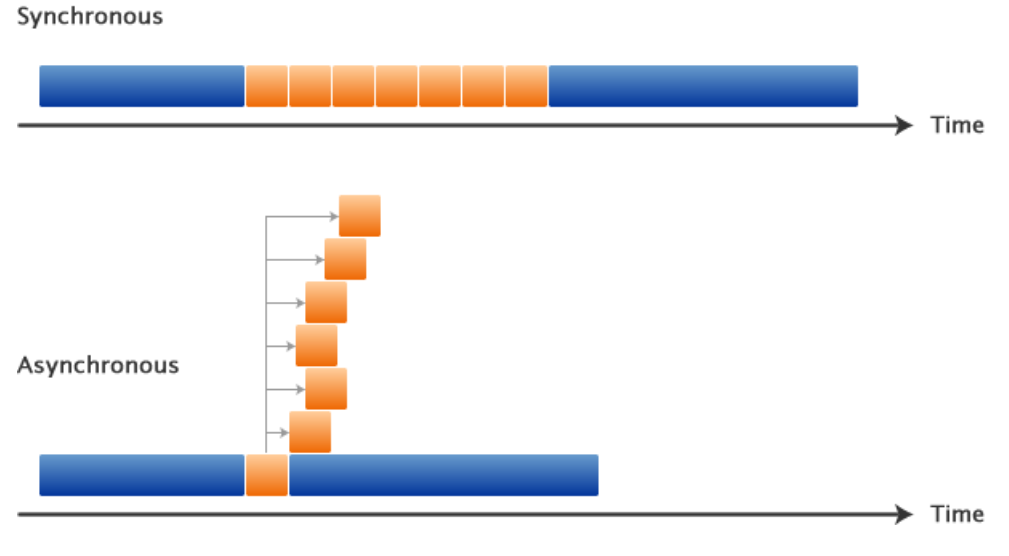
\includegraphics[width=0.8\textwidth]{img/Screenshot_20200217_112037.png}


\section{HTML Forms}

\subsection{Formulieren}
Bestaat uit 2 delen:
\begin{enumerate}
    \item Front-end: Website met formulierelementen
    \item Back-end: Verwerking op  de webserver (PHP, ASP, Python)
\end{enumerate}

\subsubsection{Front-end}
Formulieren worden gemaakt in HTML en begrensd door $<$form$>$

\begin{lstlisting}[language=HTML]
<form method="post" action="bestemming">
    <!--
    inhoud van het formulier
    tags
    velden
    -->
</form>
\end{lstlisting}

\subsubsection{Elementen}
Zie \url{http://nativeformelements.com/} of \url{https://cbracco.github.io/html5-test-page/}
\begin{itemize}
    \item Fieldset
    \item Legend
    \item Label
    \item Input
    \item Textarea
    \item Select
    \item Option
    \item Button
\end{itemize}

\subsubsection{Tekst- \& paswoordveld}
\begin{lstlisting}[language=HTML]
    <input type="text" name="veldnaam" value="inhoud veld" />
    <input type="password" name="veldnaam" value="inhoud veld" />
\end{lstlisting}

Attributen:
\begin{itemize}
    \item name
    \item id
    \item size: numeric value
    \item maxlength: numeric value
    \item value: text or numeric characters, assign an initial value to the textbox
    \item readonly: display only and cannot be edited
    \item autocomplete
    \item autofocus
    \item placeholder: text or numeric, brief info to assist the user
    \item required: value is vereist
    \item accesskey: keyboard characters
    \item tabindex: numeric, tab key order
\end{itemize}

\subsubsection{Waarom een name en een ID?}
\begin{itemize}
    \item id = identificatie van een element, kan via Javascript benaderd worden
    \item name = naam van het element, de naam waarmee de waarde doorgestuurd wordt
\end{itemize}


Tip: gebruik altijd name en ID en geef ze dezelfde waarde.
\begin{lstlisting}[language=HTML]
<input type="text" name="naam" id="naam" placeholder="Geef hier uw naam in" />
\end{lstlisting}    


\subsubsection{Label}

\begin{lstlisting}[language=HTML]
<label for="vrnm">Voornaam</label>
<input type="text" name = "vn" id="vrnm"/>
\end{lstlisting}

\begin{itemize}
    \item Label element = span met speciale functie
    \item Verplicht te gebruiken!
    \item Naar accessibility en usability toe.
\end{itemize}

\subsubsection{Textarea}
Meerdere regels invoer
\begin{lstlisting}[language=HTML]
<textarea name="commentaar" rows="4" cols="50">Hier komt de tekst</textarea>
\end{lstlisting}

\subsubsection{Select \& Option (dropdownlist)}
\begin{lstlisting}[language=HTML]
<select name="browser" size="4">
    <option value="ed">Edge</option>
    <option value="fifo">Firefox</option>
    <option value="chr">Chrome</option>
    <option value="op">Opera</option>
    <option value="an">Andere</option>
</select>
\end{lstlisting}
Multiple mogelijk $\Rightarrow$ checkbox!

\subsubsection{Optgroup}
\begin{lstlisting}[language=HTML]
<select>
    <optgroup label="Swedish cars">
        <option value="volv">Volvo</option>
        <option value ="saab">Saab</option>
    </optgroup>
    <optgroup label="German cars">
        <option value ="merc">Mercedes</option>
        <option value ="audi">Audi</option>
    </optgroup>
</select>
\end{lstlisting}
Opgepast: Label is een element \& een attribuut!

\subsubsection{Radiobuttons}
\begin{itemize}
    \item name-attribuut groepeert radiobuttons
    \item if-for zorgt voor een koppeling tussen het label en de input. 
\end{itemize}
\begin{lstlisting}[language=HTML]

<input type="radio" name="browser"id="browser1"value="FF"/>
<label for="browser1">Firefox</label><br/>

<input type="radio" name="browser"id="browser2"value="IE" checked/> 
<label for="browser2">Edge</label>

\end{lstlisting}


\subsubsection{Aankruisvakje}
\begin{itemize}
    \item name-attribuut groepeert radiobuttons
    \item if-for zorgt voor een koppeling tussen het label en de input.
\end{itemize}

\begin{lstlisting}[language=HTML]
<input type="checkbox" name="fruit[]"id="appels" value="appel" />
<label for="appels"> appels </label><br/>

<input type="checkbox" name="fruit[]"id="banaan" value="appel" />
<label for="banaan"> banaan </label>

\end{lstlisting}

\subsubsection{Fieldset/legend}
Kan gebruikt worden om een aantal controls van een formulier te groeperen door er een kader om te plaatsen.

\begin{lstlisting}[language=HTML]
<fieldset>
    <legend> Health information:</legend>
    Height: <input type="text" ... />
    Weight: <input type="text" ... />
</fieldset>
\end{lstlisting}


\subsubsection{Verzenden en reset}
\begin{itemize}
    \item value-attribuut = tekst op de knop
\end{itemize}


\begin{lstlisting}[language=HTML]
<input type="submit" value="Verzend bericht" name="verzend" />
<input type="reset" value="Wis bericht" name="wis" />

\end{lstlisting}

\subsubsection{Andere velden}
\begin{lstlisting}[language=HTML]
<input type="email" name="..." />
<input type="time" name="..." />
<input type="url" name="..." />
<input type="number" name="..." />
<input type="search" name="..." />
<input type="date" name="..." />
<input type="range" name="..." />
\end{lstlisting}

\subsection{Formulieren verzenden}
\subsubsection{Form method=GET/POST}

\begin{table}[H]
    \centering
    \resizebox{\textwidth}{!}{
    \begin{tabular}{|l|l|}
    \hline
    \bold{GET}         & \bold{POST}         \\ \hline \hline
    parameters in de url & parameters in de body \\ \hline
    gebruikt om documenten op te vragen       & gebruikt om data te wijzigen                     \\ \hline
    maximum lengte       & geen maximum lengte   \\ \hline
    OK om te cachen      & niet OK om te cachen  \\ \hline
    niet gebruiken voor wijzigen op de server & OK om te gebruiken voor wijzigingen op de server \\ \hline
    \end{tabular}
    }
\end{table}

\subsection{Valideren van een form}
Met 'required' en 'pattern'
\begin{itemize}
    \item HTML5 validate 
    \item Javascript validatie
\end{itemize}

Dit kunnen we koppelen aan CSS selectoren :valid en :invalid

\section{Flask routing}
\subsection{Backend}

Flask is een micro webframework in Python
\begin{itemize}
    \item Micro: bevat enkel de basisbenodigdheden, maar is uitbereidbaar
    \item webframework: web server gateway interface
\end{itemize}

Wij zullen Flask enkel gebruiken als backend server!

Flask is in staat om webrequests op te vangen en een response terug te sturen.
Wij zullen dit gebruiken om via webrequests json data op te vragen.

\begin{figure}[H]
    \centering
    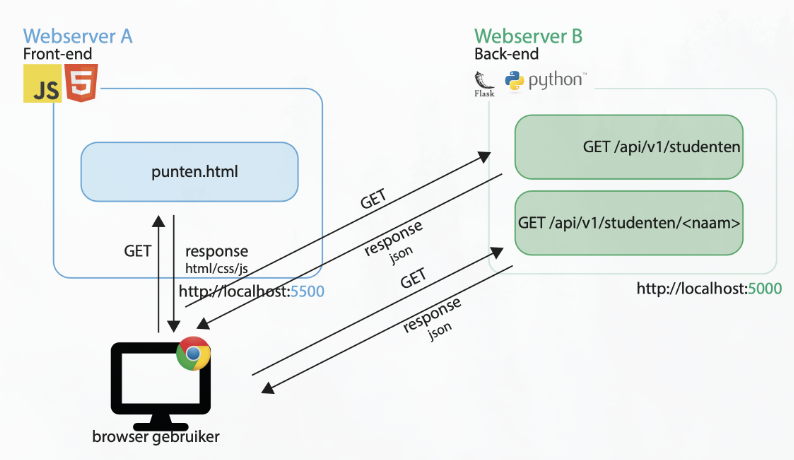
\includegraphics[width=\textwidth]{img/Screenshot_20200302_105005.png}
    \caption{Werking Flask}
\end{figure}

In de rest van de module zullen we dus gebruik maken van een\dots
\begin{itemize}
    \item Frontend server via de Live Server $\Rightarrow$ werkt op 127.0.0.1:\bold{5500}
    \item Backend server via Flask (Werkzeug) $\Rightarrow$ werkt op 127.0.0.1:\bold{5000}
\end{itemize}

Opmerkingen:
\begin{itemize}
    \item Goed opletten wat op welke poort draait, het nummer kan ook anders zijn!
    \item Voor project1 zal Live Server vervangen worden door Apache
\end{itemize}

\subsubsection{Opzetten van een Flask project in Visual Studio Code}
\begin{enumerate}
    \item Opzetten van een Virtual Environment (venv): een kopie van je python interpreter waarop je verschilllende packages installeert om de hoofdinterpreter niet te vervuilen
    \begin{itemize}
        \item Open een terminal in Visual Studio Code
        \item Ga naar de root van de FSWD-map
    \end{itemize}
    \item Typ dit in een terminal:
    \begin{lstlisting}[language=bash]
# windows
py -m venv venv_fswd
# mac/linux
python3 -m venv venv_fswd
    \end{lstlisting}
    \item Visual Studio Code zal detecteren dat je een virtual environment aanmaakt en zal je vragen dit toe te voegen aan je workspace. Doe dit!
    \item Visual Studio Code zal vragen om \bold{pylinter} toe te voegen aan je interpreter. Doe dit!
    \item Indien er een update van \bold{pip} is, installeer die update!
    \begin{itemize}
        \item \bold{pip} is de standaard package installer van python.
    \end{itemize}
\end{enumerate}

\subsubsection{Flask in python}
\begin{lstlisting}[language=python]
from flask import Flask

app = Flask(__name__) # __name__ = naam van huidige module

if __name__ == "__main__": # zal uitgevoerd worden indien dit script rechtstreeks uitgevoerd wordt (dus niet via een import vanuit een andere file)
    app.run(host='127.0.0.1', port='5000', debug=True) # debug=True zorgt ervoor dat de server opnieuw wordt gestart bij wijziging van je code.

# @ = function decorator: zal de onderstaande functie koppelen aan een pad en een method. Je kan dit vergelijken met een form method en action, standaard method is hier GET
@app.route('/')
def start():
    return "Hallokes"

# nieuwe route toevoegen
@app.route('/page2')
def naam_van_een_nieuwe_functie():
    return "Dit is een tweede pagina"

# deel van de URL variabel maken
@app.route('/page/<nr>')
def pagina(nr):
    return f"Dit is pagina {nr}"

# we kunnen een URL gebruiken om te GET'en, maar ook om te POST'en
@app.route("/getorpost", methods=['GET', 'POST'])
def getorpost():
    if request.method == 'GET':
        return "GET"
    else:
        return "POST"

# returnwaardes
@app.rotue('/')
def index():
    # return waarde, statuscode
    return jsonify({'name': Dieter, 'age': 39, 'city': 'Kortrijk'}), 200

# dataverwerking
@app.route('/showformdata', methods=['POST'])
def pagina1_fetch_json():
    naam = request.form['naam']
    voornaam = request.form['voornaam']

    persoon = {'naam': naam, 'voornaam': voornaam}

    return jsonify(persoon=persoon), 200

\end{lstlisting}

\begin{figure}[H]
    \centering
    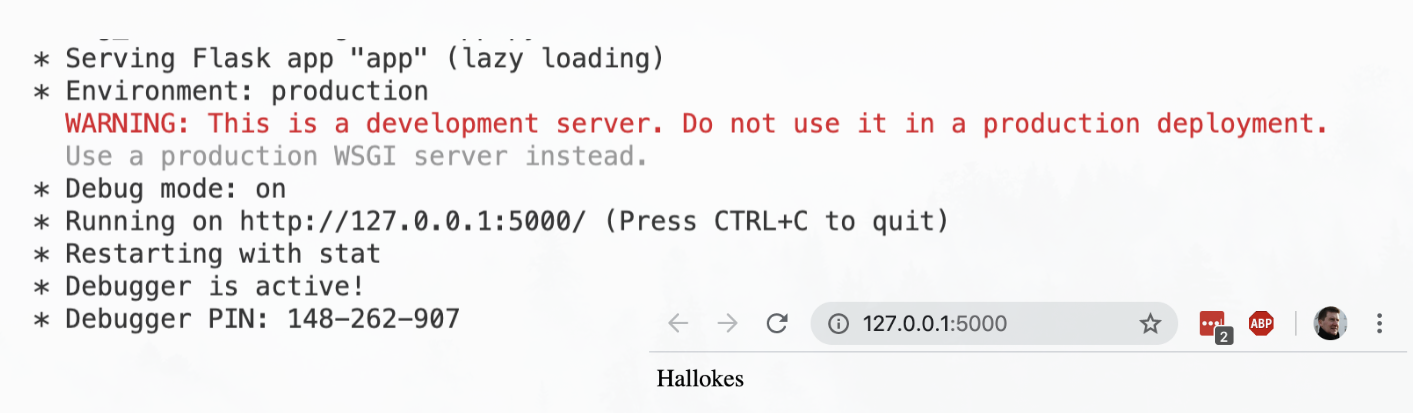
\includegraphics[width=\textwidth]{img/Screenshot_20200302_110759.png}
    \caption{Running Flask}
\end{figure}

\subsection{Frontend}
\subsubsection{Datahandler}
Om het opvragen van de data makkelijker te maken vanuit de frontend schreven we voor jullie een datahandler:


\begin{lstlisting}[language=JavaScript]
const handleData = function(url, callbackFunctionName, callbackErrorFunctionName = null, method = 'GET', body = null) {
    fetch(url, {
      method: method,
      body: body,
      headers: { 'content-type': 'application/json' }
    })
      .then(function(response) {
        if (!response.ok) {
          console.warn(`>> Probleem bij de fetch(). Statuscode: ${response.status}`);
          if (callbackErrorFunctionName) {
            console.warn(`>> Callback errorfunctie ${callbackErrorFunctionName.name}(response) wordt opgeroepen`);
            callbackErrorFunctionName(response); 
          } else {
            console.warn('>> Er is geen callback errorfunctie meegegeven als parameter');
          }
        } else {
          console.info('>> Er is een response teruggekomen van de server');
          return response.json();
        }
      })
      .then(function(jsonObject) {
        if (jsonObject) {
          console.info('>> JSONobject is aangemaakt');
          console.info(`>> Callbackfunctie ${callbackFunctionName.name}(response) wordt opgeroepen`);
          callbackFunctionName(jsonObject);
        }
      });
    /*.catch(function(error) {
        console.warn(`>>fout bij verwerken json: ${error}`);
        if (callbackErrorFunctionName) {
          callbackErrorFunctionName(undefined);
        }
      })*/
  };
\end{lstlisting}

De functie werkt met een \bold{callbackfunctie} = een functie die zal uitgevoerd worden nadat de handleData functie uitgevoerd is. 

\begin{figure}[H]
    \centering
    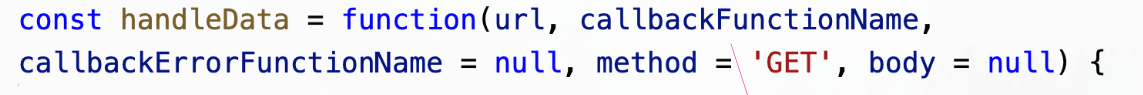
\includegraphics[width=0.7\textwidth]{img/Screenshot_20200302_111618.png}
    \caption{De callbackfunctie is de $2^{\text{de}}$ parameter van de handelData functie}
\end{figure}

\section{Flask CRUD}

\subsection{CRUD}
\begin{itemize}
    \item \bold{C}reate (of insert): toevoegen van nieuwe gegevens
    \item \bold{R}ead (of select): opvragen van gegevens
    \item \bold{U}pdate: wijzigen van gegevens
    \item \bold{D}elete: verwijderen van gegevens
\end{itemize}

In Flask gebruiken we \bold{Database.py} om de CRUD-functionaliteit te gebruiken in onze backend.

In \bold{DataRepository.py} schrijven we alle CRUD-acties:


\subsection{CRUD-acties zonder parameters}

\begin{lstlisting}[language=Python]
@staticmethod
def read_klanten():
    sql = "SELECT * FROM tblKlant"
    return Database.get_rows(sql)
\end{lstlisting}



\subsection{CRUD-acties met parameters}

\begin{lstlisting}[language=Python]
@staticmethod
def read_klant(id):
    sql = "SELECT * FROM tblKlant WHERE KlantID = %s"
    params = [id]
    return Database.get_one_row(sql, params)
\end{lstlisting}

\subsection{Andere CRUD-acties}
Andere CRUD-acties doen we met de methode Database.execute\_sql(sql, params):

\begin{lstlisting}[language=Python]
    @staticmethod
    def delete_klant(id):
        sql = "DELETE FROM tblKlant WHERE KlantID = %s"
        params = [id]
        return Database.execute_sql(sql, params)
\end{lstlisting}


\section{Dynamic eventlisteners}
Soms wil je iets tonen aan de user (zwart, rood, \dots), maar iets anders bijhouden 'achter de schermen' (\#000, \#F00, \dots).
Hiervoor gebruiken we een data-attribute (\url{https://developer.mozilla.org/en-US/docs/Learn/HTML/Howto/Use_data_attributes}).

\subsection{Data-attributes}

Data-attributes zien er in de HTML-code zo uit:

\begin{lstlisting}[language=HTML]
<ul>
    <li class="example" data-code="#000">black</li>
    <li class="example" data-code="#F00">red</li>
    <li class="example" data-code="#0F0">green</li>
    <li class="example" data-code="#00F">blue</li>
    <li class="example" data-code="#FF0">yellow</li>
    <li class="example" data-code="#0FF">cyan</li>
    <li class="example" data-code="#F0F">magenta</li>
</ul>
\end{lstlisting}

We hebben 2 mogelijkheden om deze data-attribute aan te spreken:
\begin{lstlisting}[language=JavaScript]
// met getAttribute():
this.getAttribute("data-naam");
// met het dataset variabele:
this.dataset.naam; // Let op: niet data-naam!
\end{lstlisting}

\subsection{Eventlisteners}
\underline{Voorbeeld uit de treinoefening:}

\begin{lstlisting}[language=JavaScript] 
function listenToSelectStation(){
    // selecteer alle options
    let options = document.querySelectorAll(".js-station");

    // loop over alle options
    for (let option of options) {
        // voeg voor elke option een eventlistener toe
        option.addEventListener("click", function() {
            // haal het destinationID uit de dataset:
            currentDestinationID = this.dataset.destinationId;
            // roep de getter op met de huidige destinationID
            getTrainsByDestination(currentDestinationID);
        });
    }
}
\end{lstlisting}

\section{Javascript - Support}
\subsection{URL Queryparams}
Manier om de querystring van een URL uit te lezen in JavaScript.

\begin{itemize}
    \item Vroeger kon dit enkel door gebruik te maken van reguliere expressies en string splitting functies: ingewikkeld, veel werk 
    \item Sinds Jan 2016:URLSearchParams = API: makkelijk,weinig werk
    \item Ondersteuning? \url{CanIUse.com}
\end{itemize}

\begin{lstlisting}[language=JavaScript]
// url = https://www.example.com/index.html?waarde=hallo
console.log(window.location.search) // returnt "?waarde=hallo"

// Met URLSearchParams:
const querystring = new URLSearchParams(window.location.search);
console.log(querystring.get("waarde")); // print "hallo"

//querystring.has(): returnt een boolean
if (querystring.has("waarde2")) { ... } 
\end{lstlisting}


\subsection{1 app.js voor meerdere html bestanden}
\subsubsection{Voor grote projecten:}
\begin{itemize}
    \item Gemeenschappelijke code in 1 bestand
    \item Aparte code in aparte bestanden
    \item Nadeel: code staat verspreid en is niet makkelijk te onderhouden
\end{itemize}

\subsubsection{Voor kleine projecten:}
\begin{itemize}
    \item Met een if-statement in init() die checkt welke functie op welke pagina moet worden uitgevoerd.
    \item Alle code in 1 bestand
    \item Gemeenschappelijke code bovenaan
\end{itemize}

\begin{lstlisting}[language=JavaScript]
const functie_die_ik_enkel_op_pagina1_nodig_heb = function() {
    functie_die_ik_op_elke_pagina_nodig_heb("ik word uitgevoerd op pagina 1");
};
    
const functie_die_ik_enkel_op_pagina2_nodig_heb = function() {
    functie_die_ik_op_elke_pagina_nodig_heb("ik word uitgevoerd op pagina 2");
};

const init = function() {
    if (document.querySelector(".js-pagina1")) {
        functie_die_ik_enkel_op_pagina1_nodig_heb();
    } else if (document.querySelector(".js-pagina2")) {
        functie_die_ik_enkel_op_pagina2_nodig_heb();
    }
};
\end{lstlisting}

\subsection{this vs event.target}


\begin{itemize}
    \item Het gebruik van het keyword \bold{this} bij dynamische eventhandlers:
    \begin{itemize}
        \item this = het element waarop het event getriggerd werd
    \end{itemize}
    \item Het gebruik van het \bold{event} bij dynamische eventhandlers:
    \begin{itemize}
        \item evt = alle properties en method die verband houden met het event
    \end{itemize}
\end{itemize}


\begin{lstlisting}[language=JavaScript]
const functie_die_ik_op_elke_pagina_nodig_heb = function(message) {
    document.querySelector(".js-result").innerHTML += `${message}<br/>`;
    console.log(message);
};

const doeIets = function(element) {
    functie_die_ik_op_elke_pagina_nodig_heb(element);
    element.innerHTML = "Hier heb ik reeds op geklikt.";
}; 

const doeIetsAnders = function(evt) {
    functie_die_ik_op_elke_pagina_nodig_heb(evt.target);  //het element waar op geklikt wordt
    functie_die_ik_op_elke_pagina_nodig_heb(evt.screenX); //toont waar de x-positie waar je geklikt hebt
};


const init = function() {
    let items = document.querySelectorAll(".c-container__item");

    for (const item of items) {
        item.addEventListener("click", function(e) { //belangrijk dat je 'e' meegeeft.
            //gebruik van this
            doeIets(this); //this moet niet meegegeven worden
            //gebruik van het event
            doeIetsAnders(e);
        });
    }
};
\end{lstlisting}

\section{Realtime communicatie}
\subsection{Websockets}
\begin{itemize}
    \item Websocket is een netwerkprotocol dat \underline{full-duplexcommunicatie} biedt over een \underline{TCP} verbinding
    \item Een verbinding over ws:// of wss://
    \item Om een websocket te openen wordt een speciale HTTP-request gestuurd met een \underline{'connection: upgrade'}-aanvraag
    \item Hierop stuurt de server een response met code \underline{`101 Switching Protocols'}
    \item Daarna kan er gecommuniceerd worden zonder http-request of http-responses, maar wel via zogenaamde \underline{messages}
\end{itemize}

\subsubsection{Zelf programmeren}
\begin{itemize}
    \item Kan perfect zelf, maar we kiezen voor een library
    \item \underline{Socket.io}: een javascript library en de bijhorende Python extension Flask-socketio
    \item Een gedeelte is al geschreven en we kunnen dit sneller toepassen
\end{itemize}

\subsection{Socket.io}
\subsubsection{front-end}
Laad de code van Socket.io in de header in, voor je je eigen app.js inlaadt:
\begin{lstlisting}[language=HTML]
<script src="https://cdnjs.cloudflare.com/ajax/libs/socket.io/2.3.0/socket.io.js" integrity="sha256-bQmrZe4yPnQrLTY+1gYylfNMBuGfnT/HKsCGX+9Xuqo=" crossorigin="anonymous"></script>
\end{lstlisting}

Om nu een websocket connectie naar de backend/server te openen typ je: 
\begin{lstlisting}[language=Javascript]
const lanIP = `${window.location.hostname}:5000`;
const socketio = io(lanIP);
\end{lstlisting}

Eerst halen we de huidige hostname op en plakken daar :5000 aan, zo komen we aan het adres van de backend.
Daarna openen we de connectie naar de backend met io(adres\_van\_backend)


\subsubsection{back-end}
\begin{lstlisting}[language=Python]
pip install flask-socketio
# nieuwe development server, want de flask server ondersteunt geen sockets
pip install eventlet 
\end{lstlisting}

Nu kunnen we in onze app.py de code toevoegen om een SocketIO server op te zetten:

\begin{lstlisting}[language=Python]
from flask_socketio import SocketIO, send, emit

socketio = SocketIO(app, cors_allowed_origins="*")

if __name__ == '__main__':
    # socketio heeft een wrapper waarin we de app moeten meegeven.
    # zo worden de socketio eigenschappen toegevoegd aan de app.
    # door 0.0.0.0 te gebruiken kan de server ook van buitenaf worden aangesproken.
    socketio.run(app, host="0.0.0.0", port=5000, debug=True)
\end{lstlisting}

Indien je je pythoncode nu runt, zal Python de nieuwe server (eventlet) opstarten ipv Werkzeug (de webserver van Flask). 
Je kan dit herkennen aan volgende code:

\begin{figure}[H]
    \centering
    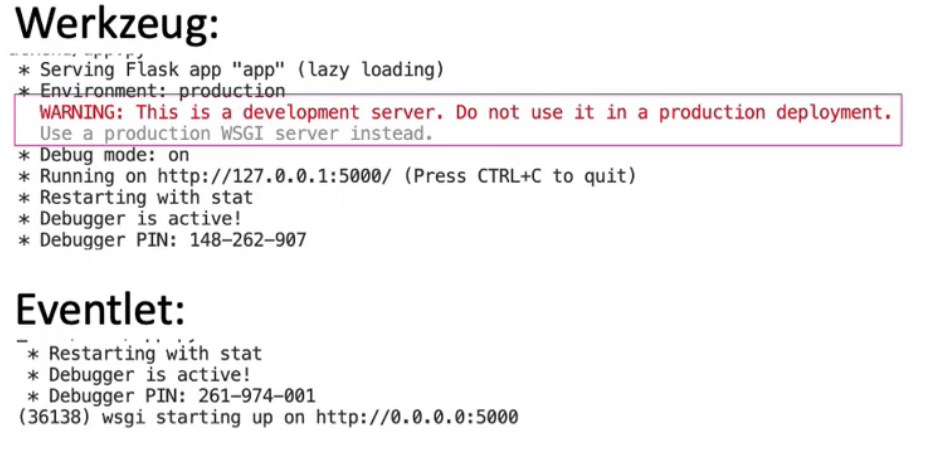
\includegraphics[width=0.9\textwidth]{img/Screenshot_20200420_085708.png} 
    \caption{Werkzeug vs Eventlet}   
\end{figure}


\subsubsection{Werking}
Hoe kan je nu 'messages' sturen van de front-end naar de backend?

Je gebruikt \bold{socketio.send} of \bold{socketio.emit} om een boodschap te versturen,
waar socketio de variabele is die onze verbinding voorstelt.

\bold{Met socketio.send:}

front-end $\Rightarrow$ back-end (in JavaScript):
\begin{lstlisting}[language=Javascript]
socketio.send("dit is een boodschap");
\end{lstlisting}

back-end $\Rightarrow$ front-end (in Python):
\begin{lstlisting}[language=Python]
socketio.send("dit is een boodschap")
\end{lstlisting}

\bold{Met socketio.emit:}

front-end $\Rightarrow$ back-end (in JavaScript):
\begin{lstlisting}[language=Javascript]
socketio.emit("naam", "dit is een boodschap");
\end{lstlisting}

back-end $\Rightarrow$ front-end (in Python):
\begin{lstlisting}[language=Python]
socketio.emit("naam", "dit is een boodschap")
\end{lstlisting}

Bij een send kunnen we enkel een string doorsturen.

$\quad\rightarrow$ eenvoudig, standaard

Bij een emit kunnen we ook een object doorsturen (payload), samen met een custom eventnaam

$\quad\rightarrow$ Meer variaties, ook objecten


\begin{figure}[H]
    \centering
    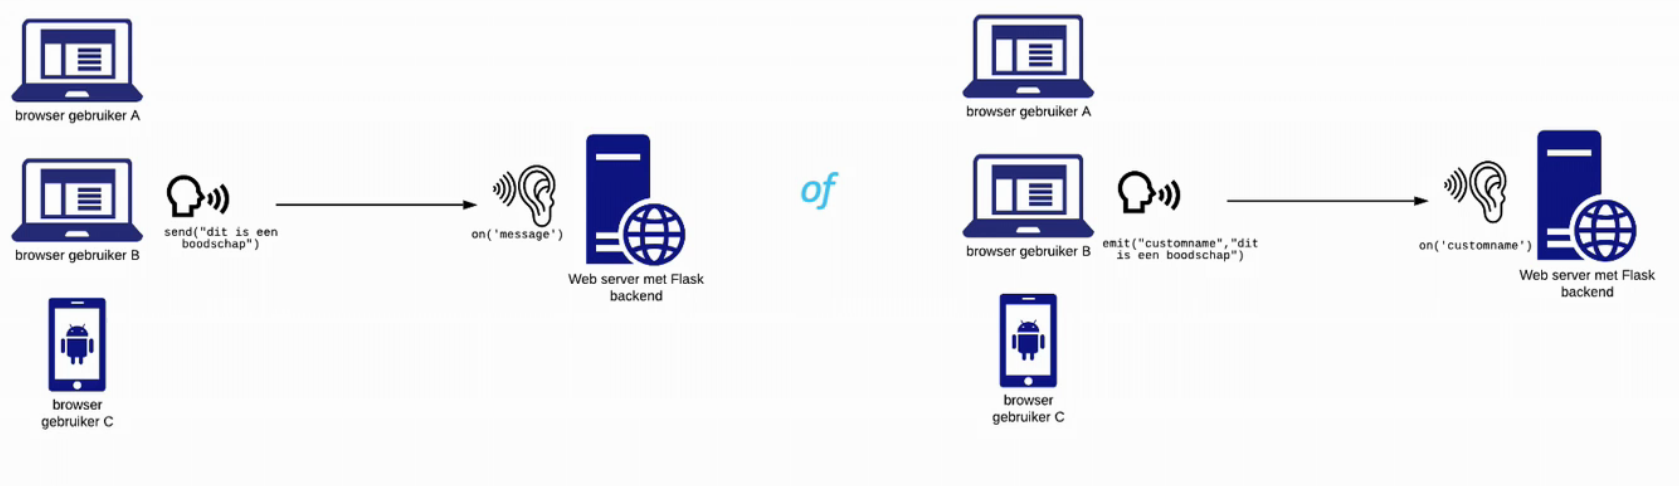
\includegraphics[width=\textwidth]{img/Screenshot_20200420_090800.png} 
    \caption{send vs emit}   
\end{figure}

\bold{Het verschil kan je goed zien bij het opvangen.}

Versturen we in de frontend (JS) de volgende code:
\begin{lstlisting}[language=Javascript]
// voor send:
socketio.send("dit is een boodschap");

// voor emit:
socketio.emit("customname", "dit is een boodschap");
\end{lstlisting}

dan moeten we die in Python ontvangen met:
\begin{lstlisting}[language=Python]
# 'message' vangt alles op dat via send binnenkomt
@socket.on('message')
def naam_functie(msg):
    print(f"{msg}")

# 'customname' vangt enkel op indien de naam 'customname' is:
@socket.on('customname')
def naam_custom_functie(msg):
    print(f"${msg}")
\end{lstlisting}


We kunnen nu boodschappen sturen van de client naar de server (client-server is altijd 1-op-1 connectie)

Indien we nu boodschappen sturen van de server naar de client kunnen we kiezen:
\begin{itemize}
    \item We sturen een boodschap naar de ene client die net een boodschap stuurde
    \item We sturen een boodschap naar alle clients die momenteel verbonden zijn (=broadcast). Dit kan zowel met send als met emit.
\end{itemize}

Server $\rightarrow$ client kan zowel 1-op-1 als 1-op-veel connectie zijn.

\begin{figure}[H]
    \centering
    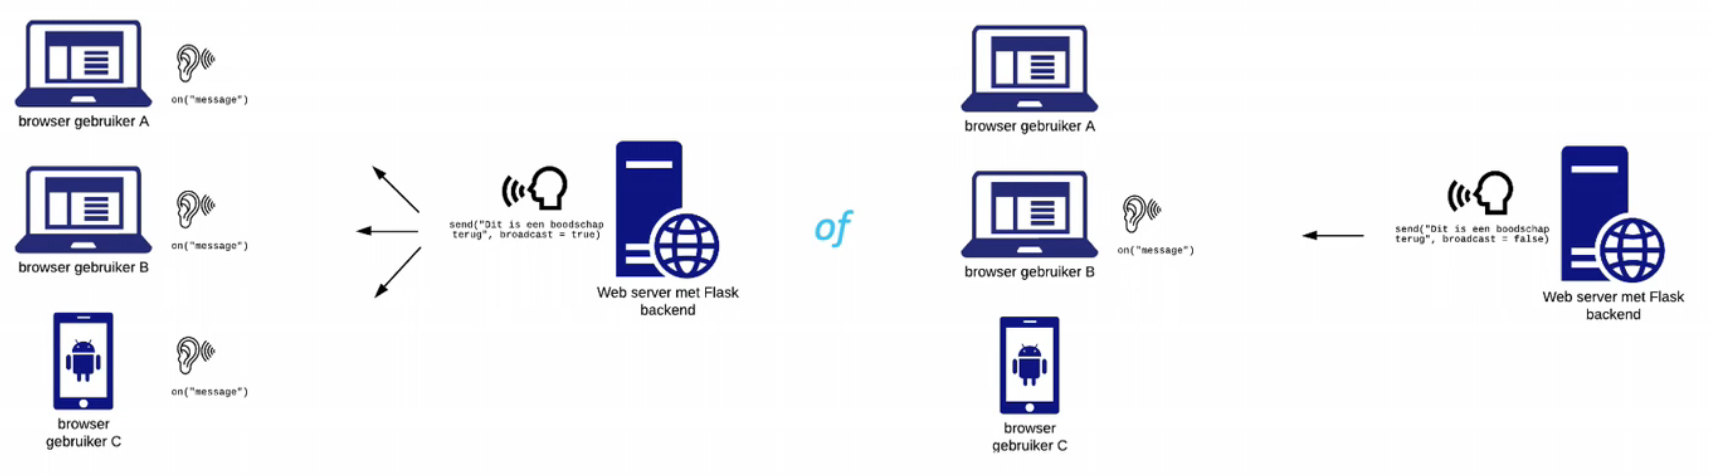
\includegraphics[width=\textwidth]{img/Screenshot_20200420_091635.png} 
    \caption{Broadcast aan of uit}   
\end{figure}

\bold{Voorbeeld:} we versturen nu eens een boodschap van server naar client(s) bij het ontvangen van een bericht:
\begin{lstlisting}[language=Python]
@socket.on('message')
def naam_functie(msg):
    print(f"{msg}")
    socketio.send("Berichtje terug", broadcast=True)
    # je kan natuurlijk ook socketio.emit() gebruiken ipv send
    # om een extra payload door te sturen
\end{lstlisting}

Alle verbonden clients zullen nu "Berichtje terug"\ ontvangen,
ze zullen dit kunnen opvangen met een socket.on("message")

\section{API authenticatie \& authorisatie met JSON web tokens}
Hoe kunnen we communicatie tussen Frontend en API beveiligen?

\bold{Authenticatie} $\Rightarrow$ Wie ben je?

\bold{Autorisatie} $\Rightarrow$ Waar heb je toegang tot?

\subsection{Verschillende authenticatietypes}
\begin{itemize}
    \item Anonymous: iedereen krijgt toegang
    \item API keys: bij elk request een API key meegeven via Authorization Header
    \begin{itemize}
        \item Bv: {“api-key”: “5742d889-4de3-4cf7-803c-ea3bff667eb9”}
    \end{itemize}
    \item Basic Authentication: Bij elk request een Base64 encoded string meegeven van username en password via de Authorization Header
    \item Token Authentication : De client, na al dan niet verificatie van paswoord/username, krijgt een toegangsticket (een token), dat vervalt na x tijd. Bij elke volgende request eeft de client dit token mee via de Authorization Header
    \begin{itemize}
        \item Veel gebruikt!
    \end{itemize}
\end{itemize}


\begin{figure}[H]
    \centering
    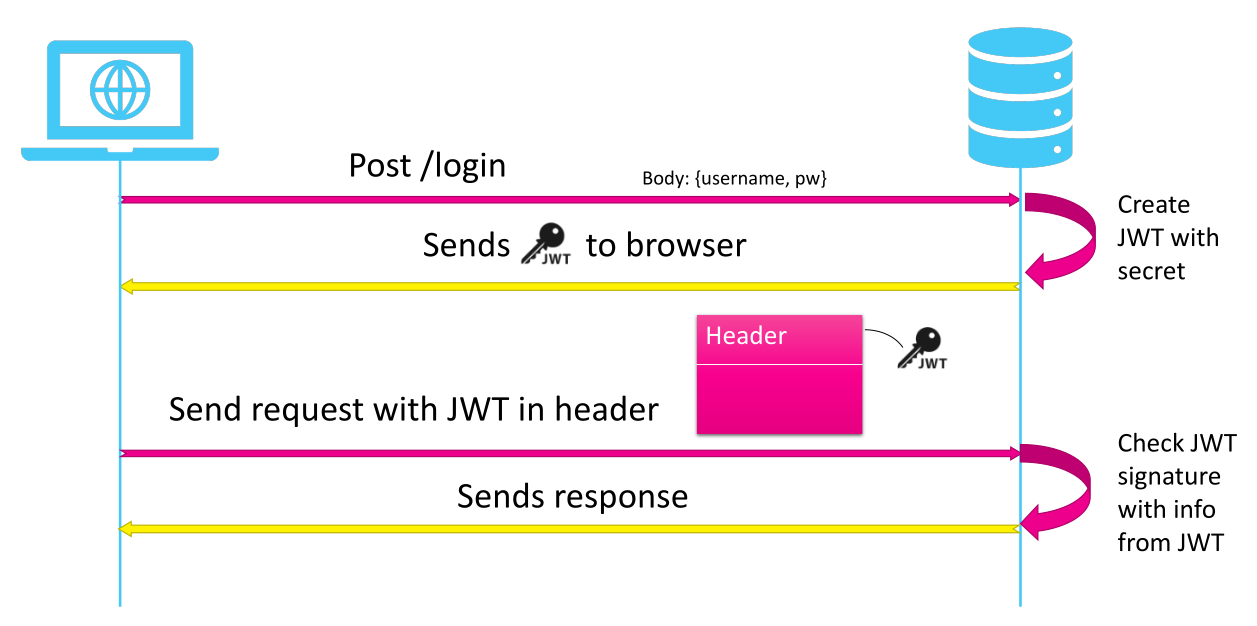
\includegraphics[width=0.8\textwidth]{img/Screenshot_20200507_202050.png}
    \caption{Token authenticatie van dichter bij bekeken}
\end{figure}

\subsection{Wat zijn JSON web tokens (JWT)?}
\begin{itemize}
    \item JSON Web Token (Industry standard RFC 7519)
    \begin{itemize}
        \item Een open standaard (RFC7519) om op een compacte en veilige manier gegevens
        tussen twee partijen uit te wisselen.
        \item Een JSON object 
        \item De informatie kan geverifieerd en vertrouwd worden door de digitale handtekening.
    \end{itemize}
    \item Een toegangsticket dat credentials en claims bevat.
    \item Wordt door client verstuurd bij elke request
    \item Bestaat uit drie delen: een \bold{header}, een \bold{payload} en een \bold{signature}
\end{itemize}

\begin{figure}[H]
    \centering
    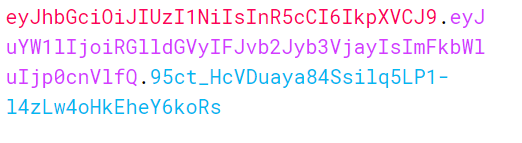
\includegraphics[width=0.5\textwidth]{img/jwt.png}
    \caption{JWT string: header, payload en signature}
\end{figure}

Met behulp van \url{http://www.jwt.io/}: illustreert het coderen, decoderen en verifiëren van een JWT ticket.
De gehashte header en gehashte payload worden samengevoegd met een punt tussen, die string wordt dan op zijn beurt samengevoegd met een gekozen secret.
De resulterende string wordt gehashed, met als resultaat de JWT signature. 

\subsubsection{JWT - Header}
De Header bevat het gebruikte encryptie algoritme en type JWT.

\begin{figure}[H]
    \centering
    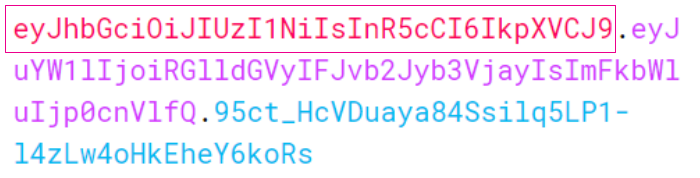
\includegraphics[width=0.5\textwidth]{img/jwt2.png}
    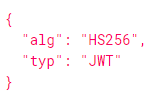
\includegraphics[width=0.2\textwidth]{img/jwt3.png}
    \caption{JWT Header}
\end{figure}


\subsubsection{JWT - Payload}
De payload bevat alle belangrijke gegevens over de gebruiker, inclusief autorisatie
rechten zoals claims en permissies.

\begin{figure}[H]
    \centering
    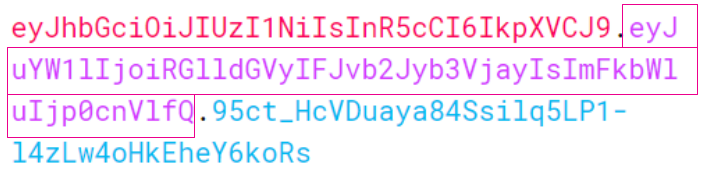
\includegraphics[width=0.5\textwidth]{img/jwt4.png}
    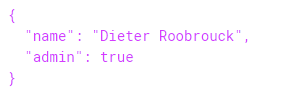
\includegraphics[width=0.3\textwidth]{img/jwt5.png}
    \caption{JWT Payload}
\end{figure}

Deze zijn voor iedereen inzichtelijk dus let erop dat je hier geen gevoelige informatie inzet!
Ook is een JWT token erop gemaakt om kort en compact te zijn dus denk aan de lengte van de namen van de
claims die je aan het token toevoegt.

\subsubsection{JWT - Signature}
De handtekening wordt gebruikt om de echtheid van het token te garanderen.
Ze bestaat uit een hash van header en payload aangevuld met een secret.

\begin{figure}[H]
    \centering
    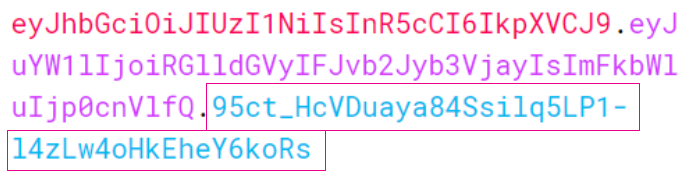
\includegraphics[width=0.5\textwidth]{img/jwt6.png}
    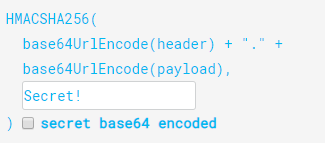
\includegraphics[width=0.3\textwidth]{img/jwt7.png}
    \caption{JWT Signature}
\end{figure}

De secret is enkel gekend door de server en wordt nooit geshared!

\subsection{API authentication using JSON Web Tokens}
\subsubsection{Stap 1: Backend (setup)}
\begin{lstlisting}[language=Python]
pip install flask-jwt-extended
\end{lstlisting}


\begin{lstlisting}[language=Python]
from flask_jwt_extended import (
    JWTManager, jwt_requird, create_access_token, get_jwt_identity
)
app.config['JWT_SECRET_KEY'] = "Secret!"
jwt = JWTManager(app)
\end{lstlisting}

\subsubsection{Stap 2: Frontend}

We willen eerst de gebruiker identificeren als geldige gebruiker door middel van een
POST-request naar de Login API-endpoint met in de payload een geldig e-mailadres en wachtwoord.

\begin{lstlisting}[language=JavaScript]
document.querySelector(".js-button").addEventListener("click", () => {
    const body = JSON.stringify({
        username: document.querySelector("#txtUsername").value,
        password: document.querySelector("#txtPassword").value
    });
    handleData('http://${lanIP}/api/v1/login', callbackShowToken, callbackShowErrorNoLogin, "POST", body);
})
\end{lstlisting}

\subsubsection{Stap 3: Backend}
\begin{enumerate}
    \item We checken of de ontvangen gegevens kloppen
    \item We maken een nieuwe JWT Token met behulp van \bold{create\_access\_token}
    \item We returnen het JWT Token terug naar de frontend
\end{enumerate}

\begin{lstlisting}[language=Python]
@app.route(endpoint + '/login', methods=['POST'])
def login():
    gegevens = DataRepository.json_or_formdata(request)

    username = gegevens['username']
    password = gegevens['password']

    #checken of de gegevens kloppen
    if username == "test" and password == "test":
        return jsonify(message="Missing username parameters"), 400
    else:
        return jsonify(message="Missing password parameters"), 400

    # normaal checken we in de usertabel of deze user bestaat 
    # en of het wachtwoord bij die user klopt, maar dit laten we even achterwege
    
    #nieuwe JWT token maken
    expires = datetime.timedelta(seconds=10)
    access_token = create_access_token(identity=username, expires_delta=expires)

    #return JWT token
    return jsonify(access_token=access_token), 200
\end{lstlisting}

\subsubsection{Stap 4: Frontend}
Bij een volgende request richting de API moet de verkregen token meegegeven
worden zodat de API de gebruiker kan verifiëren. Dit kan gedaan worden door
de \bold{Authorization header} in te vullen met de token die het login endpoint had
teruggeven:

\begin{lstlisting}[language=JavaScript]
document.querySelector(".js-button-protected").addEventListener("click", () => {
    document.querySelector(".js-result").innerHTML = "";
    handleData('http://${lanIP}/api/v1/protected', callbackShowUser, callbackShowError, "GET", null, token); //token = Authorization header
});
\end{lstlisting}

* Daarvoor gaan we onze dataHandler moeten uitbreiden. Zie demo.

\subsubsection{Stap 5: Backend}
\begin{enumerate}
    \item We beveiligen onze endpoint door een decorator toe te voegen: \lstinline{@jwt_required}
    \item We kunnen ook de identiteit opvragen van het token door middel van \lstinline{get_jwt_identity}
    \item We retourneren een response terug
\end{enumerate}

\begin{lstlisting}[language=Python]
@app.route(endpoint + "/protected", methods=["GET"])
@jwt_required
def protected():
    current_user = get_jwt_identity()
    return jsonify(logged_in_as=current_user), 200
\end{lstlisting}

Volledige uitleg: zie demo

\section{Threading}
Normaal wordt code van boven naar onder uitgevoerd. 
De volgende lijn van je programeercode kan slechts worden uitgevoerd als de bovenstaande lijn code is afgerond.

Met threading kunnen we ervoor zorgen dat code naast elkaar (asynchroon) kan worden uitgevoerd.

\subsection{threading.Thread(target=callbackfunction)}


\begin{lstlisting}[language=Python]
    def zeg_hello():
    #zeg 6 maal hello maar wacht 2 seconden tussen elke boodschap
    for i in range(6):
        print(f"Hello student {i}")
        time.sleep(2)

mijn_ander_proces = threading.Thread(target=zeg_hello)
mijn_ander_proces.start()

print('veeg het bord af')
print('start de pc op')
print('start de beamer op')
print('ga naar leho')
\end{lstlisting}

\subsubsection{Output}

\begin{lstlisting}
Hello student 0
veeg het bord af
start de pc op
start de beamer op
ga naar leho
Hello student 1
Hello student 2
Hello student 3
Hello student 4
Hello student 5
\end{lstlisting}

\subsection{threading.Timer(seconds, callbackfunction)}

threading.Timer() wacht eerst 3 seconden, en roept dan de callbackfunctie op:

\begin{lstlisting}[language=Python]
import time
import threading
def zeg_hello():
    #zeg 6 maal hello maar wacht 2 seconden tussen elke boodschap
    for i in range(6):
        print(f"Hello student {i}")
        time.sleep(2)

mijn_ander_proces = threading.Timer(3,zeg_hello)
mijn_ander_proces.start()
print('veeg het bord af')
time.sleep(1)
print('start de pc op')
time.sleep(1)
print('start de beamer op')
time.sleep(1)
print('ga naar leho')
time.sleep(1)
\end{lstlisting}

\subsubsection{Output}

\begin{lstlisting}[]
veeg het bord af
start de pc op
start de beamer op
Hello student 0
ga naar leho
Hello student 1
Hello student 2
Hello student 3
Hello student 4
Hello student 5
\end{lstlisting}






\end{document}

